% =====================================================================
% WoodID-S2-2026 — assembly file for the Person-3 sections
%
% Compile from the REPOSITORY ROOT so that the \includegraphics paths
% (artifact/person3/..., artifact/person1/...) resolve:
%
%     pdflatex -output-directory=paper_draft_person3/build \
%              paper_draft_person3/main.tex
%
% Sections 1 (Introduction) and 3 (Materials and Methods) are owned by
% other authors and are not included here; the \input lines for them are
% left commented so this file compiles standalone.
%
% LAYOUT. One-column arXiv/NeurIPS-style preprint: letter paper, a
% 5.5in x 9in text block, Times, arabic section numbers with no trailing
% period, an abstract indented on both sides, and "Table 1:" / "Figure 1:"
% captions. All of that lives in paper_draft_person3/woodid.sty, which the
% Vietnamese build loads too, so the two versions cannot drift apart.
% Every table and figure is an ordinary float -- no starred floats.
% =====================================================================
\documentclass[10pt]{article}
% Tim woodid.sty trong thu muc cua chinh bai bao. Nho dong nay, lenh
% \usepackage duoi day chay duoc du bien dich tu thu muc goc repo
% (cach dung dung, vi duong dan anh la tuong doi so voi goc) hay tu
% trong paper_draft_person3/.
\makeatletter
\providecommand{\input@path}{}
\edef\input@path{{paper_draft_person3/}{./}\input@path}
\makeatother
\usepackage{woodid}

\begin{document}

\title{A Systematic Benchmark of Deep Learning Architectures for Conifer
Wood Species Identification Using Macroscopic Cross-Section Images}
\author{WoodID-S2-2026}
\maketitle

% =====================================================================
% Section 0 — Abstract
%
% Written last, after Sections 4, 5 and 6 were complete.
% CONSTRAINT: every number here already appears in Section 4. No result is
% introduced that is not reported in Results.
%
%   92.356 +/- 1.022   Table 1 (tab:task_b)
%   99.561 +/- 0.354   Table 1 (tab:task_b)
%   98.371 +/- 0.319   Table 1 (tab:task_b)
%   1.19 points        Sec 4.6
%   4.22 M / 27.83 M   Table 4 (tab:efficiency)
%   61 vs 1            Sec 4.3
%   95.3 / 96.6 / 37.970  Sec 4.5
%   17 species, 532 test images, 3 seeds  Sec 4.1
% =====================================================================

\begin{abstract}
Macroscopic cross-section imaging is the most deployable route to conifer
wood identification, but it is unclear which modern architecture it calls
for, or how much of the reported accuracy reflects anatomical evidence. We
benchmark ResNet-50, EfficientNet-B3, MobileNetV3-Large, ConvNeXt-Tiny and
Swin-Tiny on 17 conifer species, using a partition grouped by origin key,
three seeds per configuration, and a single immutable evaluation registry.
Results are reported as mean and standard deviation across seeds; no
interval estimate is claimed.

ResNet-50 is not competitive, reaching $92.356 \pm 1.022$\,\% test accuracy
against $99.561 \pm 0.354$\,\% for ConvNeXt-Tiny, and producing 122 of the
204 errors made by all backbones and seeds combined. The remaining four
architectures are separated by margins comparable to their seed-to-seed
variation, so three seeds do not establish their ordering.
MobileNetV3-Large is the practically notable case, reaching
$98.371 \pm 0.319$\,\% with 4.22\,M parameters against 27.83\,M. Errors are
concentrated: in the strongest model every error is the same confusion
between \textit{Pinus krempfii} and \textit{Pinus dalatensis}, a pair
present in all five architectures and asymmetric at 61 occurrences against
one reversed. Two augmentation ablations were each trained with a single
seed and support no recommendation.

A control experiment qualifies these numbers. Models trained on
$16\times16$ or heavily blurred inputs retain 95.3\,\% and 96.6\,\% of
full-image accuracy, while a colour-histogram-only model reaches
37.970\,\%. Since anatomical structure does not survive those
transformations, the accuracies reported here describe performance on this
corpus rather than anatomical identification, and external validation
remains the necessary next step.
\end{abstract}

\begin{paperkeywords}
wood identification, conifer species, macroscopic cross-section, deep
learning benchmark, shortcut learning, dataset leakage
\end{paperkeywords}


% \input{sections/01_introduction}     % other author
% \input{sections/02_related_work}     % other author
% \input{sections/03_materials_methods}% other author

% =====================================================================
% Section 4 — Experimental Results
%
% PROVENANCE. Every quantitative statement in this section resolves to a
% table or figure, and every table or figure resolves to the immutable
% registry below. Nothing here is quoted from an earlier report.
%
%   Registry   : docs/reports/experiments/phase_1b/final_b_new_recomputed/
%                20260819T043733Z/
%   Created    : 2026-08-19T04:37:33.586402+00:00
%   Git commit : 75df6c061eca5a3d63cfac706d1b6e256e404342
%   Split      : task-B-group-split:359be7f5379818d4
%
%   tab:task_b           <- main_test_summary.csv        (15 runs)
%   tab:ablation         <- ablation_vs_main_seed42.csv  (20 runs)
%   tab:perspecies_full  <- per_class_metrics.csv        (15 runs)
%   fig:confusion        <- predictions.csv              (3 runs)
%   fig:perclass         <- per_class_metrics.csv        (15 runs)
%
% NGOAI REGISTRY (nguon khac, lineage rieng -- ghi ro trong tung caption):
%   tab:efficiency  <- results/efficiency.csv
%                      thuoc tinh kien truc, do voi pretrained=False;
%                      latency da bo (do tren RTX 3060, khac phan cung registry)
%   Sec 4.5 probe   <- docs/reports/experiments/phase_1b/anatomy_destruction_probe/
%                      tables/anatomy_probe_summary.csv + run_summary.json
%   Sec 4.5 hoi tu  <- data/experiments/Task-B-new/final/**/test_metrics.json
%                      (best_epoch / epochs_trained / stopped_early / final acc)
%   fig:gradcam     <- artifact/person1/gradcam/  (repo WoodID, branch p1,
%   fig:tsne        <- artifact/person1/tsne/      commit d39a3f6; xem SOURCE.txt)
%                      ca hai dung checkpoint seed 42 cua CUNG registry nay
%
% Per-table run-id lists are carried in artifact/person3/tables/
% tables_metadata.json and in the header comment of each .tex file.
%
% REPORTING RULE. Dispersion is always a standard deviation over the three
% main seeds. It is never an interval estimate, and no claim of statistical
% reliability is attached to any difference in this section.
% =====================================================================

\section{Experimental Results}
\label{sec:results}

\subsection{Experimental Setup}
\label{sec:results:setup}

All runs reported in this section come from a single immutable evaluation
registry, created on 2026-08-19 against git commit
\texttt{75df6c06} and split version
\texttt{task-B-group-split:\allowbreak 359be7f5379818d4}. Re-running the evaluation
notebook against that commit reproduces every number below.

\paragraph{Data.} The Task~B partition contains 17 conifer species split
3{,}365 / 903 / 532 images across train / validation / test. Three further
species present in the source collection
(\textit{Calocedrus} sp., \textit{Cupressus funebris},
\textit{Pinus} sp.) were excluded because they are identified only to genus.
The partition is grouped by \emph{origin key}: images sharing an origin key
are assigned to a single split, rather than being divided image-by-image. The
origin key is derived from the filename and is intended to stand for the
physical wood specimen, so that test images come from specimens the model has
not seen rather than from unseen crops of familiar specimens. Whether the key
corresponds one-to-one to a physical specimen has not been established, and
Section~\ref{sec:discussion:originkey} sets out what the grouping does and
does not guarantee.

\paragraph{Family assignment.} Species are grouped into five families ---
Araucariaceae, Cupressaceae, Pinaceae, Podocarpaceae and Taxaceae --- following
accepted conifer taxonomy, so that \textit{Araucaria araucana} is assigned to
Araucariaceae. This differs from the four-family scheme of the project's
family-level task, which folds that species into Pinaceae. Family membership
affects only how results are grouped for presentation; it plays no part in
training or evaluation, and every per-species number is unchanged by the
choice. Family-level error rates in this section are computed under the
five-family scheme throughout.

\paragraph{Training configuration.} All five backbones were initialised from
ImageNet weights and fine-tuned for 50 epochs with a cosine schedule, a head
learning rate of $1\times10^{-4}$, a backbone learning rate of
$1\times10^{-5}$, weight decay $1\times10^{-4}$, label smoothing 0.1, and
mixed-precision training. These settings are identical across all 30
registered runs. Batch size is the one setting that varies, and it varies by
backbone rather than by experiment: 64 for ResNet-50 and MobileNetV3-Large,
32 for EfficientNet-B3, ConvNeXt-Tiny and Swin-Tiny, held constant for a
given backbone across the main runs and all three ablations. Comparisons
between an ablation and its baseline are therefore within-backbone and
single-variable; comparisons \emph{between} backbones carry batch size as an
additional uncontrolled difference.

\paragraph{Seeds and evaluation.} The main configuration was trained with
three seeds (42, 123, 456), giving 15 main runs. Each ablation was trained
with seed 42 only, giving 5 runs per ablation. Evaluation used FP16
autocast, TF32 matrix multiplication and channels-last memory format on an
NVIDIA GeForce RTX 4090 under PyTorch 2.11.0+cu128, with the whole split
resident on the GPU so that batching does not affect the result.

\subsection{Main Benchmark}
\label{sec:results:benchmark}

Table~\ref{tab:task_b} reports test accuracy and macro-F1 for the five
architectures, as the mean and standard deviation over the three main seeds.

The two modern backbones lead. ConvNeXt-Tiny reaches
$99.561 \pm 0.354$\,\% accuracy and $99.596 \pm 0.326$\,\% macro-F1,
ahead of Swin-Tiny at $99.123 \pm 0.581$\,\% and
$99.196 \pm 0.533$\,\%. MobileNetV3-Large follows at
$98.371 \pm 0.319$\,\% accuracy despite being the smallest model in the
comparison, and EfficientNet-B3 at $97.807 \pm 0.319$\,\%. ResNet-50 is
last by a clear margin, $92.356 \pm 1.022$\,\% accuracy and
$92.569 \pm 0.982$\,\% macro-F1 --- roughly seven points below the leader
and with the largest seed-to-seed spread of the five.

Two features of the spread are worth stating before any ranking is read too
firmly. First, the gaps separating ConvNeXt-Tiny, Swin-Tiny and
MobileNetV3-Large are of the same order as the seed-to-seed standard
deviations themselves, so the ordering among those three rests on
differences that a different choice of seeds could plausibly reorder.
Second, ResNet-50's separation from the rest is several times its own
standard deviation and is the one ordering in the table that does not depend
on that caveat.

Accuracy and macro-F1 track each other closely for every backbone, which is
expected given that the test partition is close to balanced --- per-species
support ranges from 24 to 39 images (Table~\ref{tab:perspecies_full}). No
backbone is buying accuracy by neglecting a small class.

\subsection{Per-Species and Confusion Analysis}
\label{sec:results:perspecies}

\paragraph{Model selection.} The confusion matrix is reported for a single
architecture, selected by a criterion fixed before the confusion structure
was inspected: the backbone with the highest mean macro-F1 over the three
main seeds, which is ConvNeXt-Tiny (Table~\ref{tab:task_b}). The
alternative of reporting whichever individual run scored highest was
rejected, and is in any case ill-defined here: seeds 42 and 123 tie exactly
at 99.812\,\% accuracy with no stated tie-break.

\paragraph{Aggregation.} Figure~\ref{fig:confusion} sums the three per-seed
$17\times17$ count matrices element-wise, giving $532\times3 = 1{,}596$
predictions. Each seed contributes equally, and row normalisation divides by
the row total of the summed counts. The per-seed matrices are published
alongside the aggregate so the sum can be checked.

\paragraph{Result.} ConvNeXt-Tiny makes 7 errors in 1{,}596 predictions, and
all 7 are the same confusion: \textit{Pinus krempfii} predicted as
\textit{Pinus dalatensis}. The matrix is otherwise exactly diagonal. Both
species are Pinaceae, so no error crosses a family boundary.

Figure~\ref{fig:perclass} and Table~\ref{tab:perspecies_full} give per-species
F1 for all five backbones. Three patterns stand out.

\textit{First}, the \textit{P.\ krempfii} / \textit{P.\ dalatensis} pair is
the only confusion that appears in every architecture: 18, 12, 15, 9 and 7
occurrences for ResNet-50, EfficientNet-B3, MobileNetV3-Large, Swin-Tiny and
ConvNeXt-Tiny respectively, 61 in total, against a single occurrence in the
reverse direction. It accounts for 61 of the 204 errors made by all
backbones and seeds combined, and it does not diminish as capacity
increases. Both species are \textit{Pinus} (Pinaceae) with comparable test
support (36 and 32 images), so neither class imbalance nor a family boundary
explains it. These two species also carry the largest seed-to-seed standard
deviation within the two strongest columns --- 3.30 to 4.08 points, against
zero for every other species under ConvNeXt-Tiny --- so the magnitude of the
effect is itself unstable.

\textit{Second}, the errors are not evenly distributed across
architectures. ResNet-50 alone produces 122 of the 204 errors. Its worst
case is \textit{Podocarpus pilgeri}, at $61.994 \pm 9.598$\,\% F1 ---
33.4 points below the next-worst model and the largest dispersion of any
cell in Table~\ref{tab:perspecies_full} --- driven by 48 confusions with
\textit{Chamaecyparis obtusa}. The remaining four architectures score
between 95.420 and 100.000\,\% F1 on the same species, and two of them make
this error zero times. Pooling architectures would present this as the
second-largest difficulty in the dataset; disaggregated, it is one model's
failure mode on this configuration and is not evidence that the two woods
resemble one another.

\textit{Third}, family-level difficulty does not follow the intuition that
the largest family is the hardest. Error rates by true family are
1.56\,\% for Araucariaceae, 0.78\,\% for Cupressaceae, 2.83\,\% for
Pinaceae, 10.93\,\% for Podocarpaceae and 7.69\,\% for Taxaceae.
Cupressaceae, the largest family at eight species, is the \emph{lowest} of
the five, and all eight of its species are error-free under ConvNeXt-Tiny.
Three of the five families contain exactly one species (Araucariaceae,
Podocarpaceae, Taxaceae), so their rates are single-species rates over much
smaller denominators and are not comparable in kind with the eight-species
and six-species rates. Excluding ResNet-50 changes the picture again:
Araucariaceae falls to 0.00\,\%, Podocarpaceae to 2.08\,\% and Taxaceae to
3.53\,\%, while Cupressaceae reaches 0.49\,\% and Pinaceae 2.13\,\%. Three
of the five families therefore owe most of their apparent difficulty to a
single backbone, and the ordering among the remaining families is not stable
between the two groupings.

\subsection{Rotation and Label Smoothing}
\label{sec:results:ablation}

Table~\ref{tab:ablation} reports three ablations against the main
configuration at the same seed and the same backbone: discrete
$90^\circ$ rotation in place of continuous $\pm30^\circ$ rotation, and label
smoothing set to 0.0 and 0.2 in place of 0.1. Each ablation was trained with
seed 42 only, so every entry is a single-run point estimate with no
dispersion of its own.

Discrete $90^\circ$ rotation does not produce a consistent effect. Its
accuracy deltas are $+0.940$, $+1.316$, $0.000$, $-0.564$ and $-0.564$
percentage points for ResNet-50, EfficientNet-B3, MobileNetV3-Large,
ConvNeXt-Tiny and Swin-Tiny --- positive for the two weaker convolutional
backbones, zero for one, and negative for both of the strongest models. The
sign is not stable across architectures, and four of the five magnitudes lie
within about 1.6 times the corresponding seed-to-seed standard deviation
from Table~\ref{tab:task_b}. Only EfficientNet-B3 shows a delta clearly
larger than its own seed noise, at roughly four times that standard
deviation, and with one seed it cannot be separated from a favourable draw.

Removing label smoothing entirely ($0.0$) lowers accuracy for all five
backbones: $-0.376$, $-0.752$, $-0.376$, $-0.188$ and $-0.188$ percentage
points. The individual magnitudes are small --- three of the five are below
the corresponding seed-to-seed standard deviation --- but the direction is
the same in all five cases, which is the only consistent pattern in the
ablation table. Raising label smoothing to $0.2$ produces no such
consistency: two backbones improve or stay level and three decline.

Taken together, neither ablation supports a recommendation. The rotation
result argues against treating discrete $90^\circ$ augmentation as a general
improvement for this task, and the label-smoothing sweep suggests that the
default of 0.1 is at least not worse than either neighbour tested. Both
readings are limited by the single-seed design
(Section~\ref{sec:discussion:oneseed}).

\subsection{Training Convergence and Anatomical Sufficiency}
\label{sec:results:convergence}

\paragraph{Convergence.} Per-epoch curves were not persisted for the registry
runs, so convergence is characterised from the summary fields recorded with
each checkpoint. The two strongest backbones converge in roughly a third of
the budget: the best validation epoch averages 20.3 for ConvNeXt-Tiny and
15.0 for Swin-Tiny, against 40.3--44.0 for MobileNetV3-Large,
EfficientNet-B3 and ResNet-50. Early stopping fired in all three seeds for
ConvNeXt-Tiny and Swin-Tiny and in none for ResNet-50. The gap between final
training and final validation accuracy separates the same two groups: 0.17
and 0.48 points for ConvNeXt-Tiny and Swin-Tiny against 3.14, 3.85 and 4.73
for the other three. The ordering by convergence speed and by generalisation
gap therefore matches the ordering by test accuracy in
Table~\ref{tab:task_b}.

\paragraph{Anatomical sufficiency.} A control experiment tests whether the
task actually requires anatomical detail. Three probes were trained on the
same partition and evaluated once on the same test set: \textbf{B1}, images
downsampled to $16\times16$ and resized back to $224\times224$; \textbf{B2},
images blurred with a Gaussian kernel of size 49 and $\sigma=8$; and
\textbf{B3}, a small multi-layer perceptron given only a normalised
$3\times32$-bin RGB histogram, discarding all spatial structure. B1 and B2
use a freshly initialised ImageNet-pretrained Swin-Tiny; the full-image
reference is the corresponding Swin-Tiny run at 99.060\,\% accuracy.

\begin{center}
\small
\begin{tabular}{llcc}
\toprule
\textbf{Probe} & \textbf{Input} & \textbf{Accuracy (\%)} & \textbf{Retention (\%)} \\
\midrule
Uniform chance      & none                        & 5.882  & --- \\
Majority class      & none                        & 7.331  & --- \\
Full image          & $224\times224$              & 99.060 & 100.0 \\
B1                  & $16\times16$ upsampled      & 94.361 & 95.3 \\
B2                  & Gaussian blur $\sigma=8$    & 95.677 & 96.6 \\
B3                  & RGB histogram only          & 37.970 & 38.3 \\
\bottomrule
\end{tabular}
\end{center}

At $16\times16$ every structure a wood anatomist would use --- tracheid
diameter, resin canals, ray cells, growth-ring boundaries --- is destroyed,
yet accuracy retains 95.3\,\% of the full-image reference. Heavy blurring
retains 96.6\,\%. Colour alone is not sufficient: B3 reaches 37.970\,\%,
well above the 5.882\,\% chance level but far below either spatial probe.
The task as posed is therefore largely solvable from low-frequency image
content that survives the destruction of anatomical detail, and the
$99$\,\%-level accuracies in Table~\ref{tab:task_b} cannot be read as
evidence that the models perform anatomical identification.
Section~\ref{sec:discussion:shortcut} takes up what this implies.

\subsection{Model Complexity}
\label{sec:results:efficiency}

Table~\ref{tab:efficiency} reports parameter count, multiply--accumulate
operations and model size at the $224\times224$ input resolution.

The accuracy ranking does not follow model size. MobileNetV3-Large reaches
$98.371 \pm 0.319$\,\% accuracy (Table~\ref{tab:task_b}) with 4.22\,M
parameters and 0.22\,G MACs --- roughly one sixth the parameters and one
twentieth the compute of ConvNeXt-Tiny, for a difference of 1.19 accuracy
points. ResNet-50, at 23.54\,M parameters and 4.13\,G MACs, is within 15\,\%
of ConvNeXt-Tiny's compute yet scores seven points lower, so the gap between
them is not explained by capacity. ConvNeXt-Tiny and Swin-Tiny are nearly
identical in complexity (27.83 versus 27.53\,M parameters, 4.46 versus
4.37\,G MACs), which makes their accuracy difference a comparison of
architecture rather than of scale.

Two limits apply to this table. Inference latency is not reported: the
available measurements were taken on different hardware from the training
and evaluation runs, so they cannot be placed alongside any other number in
this paper. And the complexity figures are architecture properties measured
on randomly initialised models, so unlike every other table here they do not
derive from the evaluation registry.

\subsection{Grad-CAM and Feature-Space Structure}
\label{sec:results:gradcam}

\paragraph{Grad-CAM.} Figure~\ref{fig:gradcam} shows Grad-CAM maps for
ConvNeXt-Tiny, Swin-Tiny and MobileNetV3-Large on five test images. The
images were selected by a rule fixed in advance: among images classified
correctly by all three models, the one nearest the median ConvNeXt-Tiny
confidence for its family, with ties broken by image path. No image was
chosen for the appearance of its heatmap. All three maps come from the
seed-42 checkpoints of the same runs used in
Table~\ref{tab:task_b}.

The attributions are diffuse and distributed across the field rather than
concentrated on identifiable anatomical landmarks, and the three
architectures highlight different regions of the same image. Read together
with the probes of Section~\ref{sec:results:convergence}, this is what would
be expected if the decisive evidence were low-frequency and spread over the
image rather than carried by localised anatomical features. Grad-CAM shows
where gradient support lies; it does not by itself establish what feature is
being used, and no anatomical reading of these maps is offered here.

\paragraph{Feature space.} Figure~\ref{fig:tsne} embeds the 768-dimensional
pre-logit features of ConvNeXt-Tiny seed 42 for all 532 test images, reduced
by PCA to 50 dimensions and then by t-SNE to two, with perplexity 30 and a
fixed random seed. Species form largely separated clusters, consistent with
the near-diagonal confusion matrix of Figure~\ref{fig:confusion}. The one
structure that matters for interpretation is the relationship between
\textit{Pinus krempfii} and \textit{Pinus dalatensis}, the single pair that
survives in the best model (Section~\ref{sec:results:perspecies}).

The embedding is a projection chosen to preserve local neighbourhoods, and
distances in it are not metric; it is included as a qualitative view of the
representation, not as evidence of separability.


% ---- tables and figures referenced by Section 4 ----
% Table: Task B main benchmark (species-level, 17 classes)
% AUTO-GENERATED bang scripts/person3/make_result_tables.py -- khong sua tay
% Source file      : docs/reports/experiments/phase_1b/final_b_new_recomputed/20260819T043733Z/main_test_summary.csv
% Registry created : 2026-08-19T04:37:33.586402+00:00
% Source run ids   : 15 runs
%   taskB17__main__seed_123__convnext_tiny
%   taskB17__main__seed_123__efficientnet_b3
%   taskB17__main__seed_123__mobilenetv3_large
%   taskB17__main__seed_123__resnet50
%   taskB17__main__seed_123__swin_tiny
%   taskB17__main__seed_42__convnext_tiny
%   taskB17__main__seed_42__efficientnet_b3
%   taskB17__main__seed_42__mobilenetv3_large
%   taskB17__main__seed_42__resnet50
%   taskB17__main__seed_42__swin_tiny
%   taskB17__main__seed_456__convnext_tiny
%   taskB17__main__seed_456__efficientnet_b3
%   taskB17__main__seed_456__mobilenetv3_large
%   taskB17__main__seed_456__resnet50
%   taskB17__main__seed_456__swin_tiny
\begin{table}[!htbp]
\centering
\caption{Species-level classification performance on the Task B test set
(17 species, 532 images, partitioned by origin key
so that images sharing an origin key fall in a single split).
Values are the mean $\pm$ standard deviation across 3 training seeds
(42, 123, 456); the spread is reported as a standard deviation over
three runs and is not an interval estimate. Best value per column in bold.}
\label{tab:task_b}
\begin{tabular}{lcc}
\toprule
\textbf{Architecture} & \textbf{Top-1 Accuracy (\%)} & \textbf{Macro-F1 (\%)} \\
\midrule
ResNet-50         & $92.356 \pm 1.022$ & $92.569 \pm 0.982$ \\
EfficientNet-B3   & $97.807 \pm 0.319$ & $97.844 \pm 0.322$ \\
MobileNetV3-Large & $98.371 \pm 0.319$ & $98.448 \pm 0.345$ \\
ConvNeXt-Tiny     & $\mathbf{99.561 \pm 0.354}$ & $\mathbf{99.596 \pm 0.326}$ \\
Swin-Tiny         & $99.123 \pm 0.581$ & $99.196 \pm 0.533$ \\
\bottomrule
\end{tabular}
\end{table}

% Table: Task B ablations vs main seed 42 (same backbone)
% LUU Y: moi ablation chi co 1 seed (42) -> khong co +/- , chi la diem don.
% AUTO-GENERATED bang scripts/person3/make_result_tables.py -- khong sua tay
% Source file      : docs/reports/experiments/phase_1b/final_b_new_recomputed/20260819T043733Z/ablation_vs_main_seed42.csv
% Registry created : 2026-08-19T04:37:33.586402+00:00
% Source run ids   : 15 runs
%   taskB17__taskB_90rotation__seed_42__convnext_tiny
%   taskB17__taskB_90rotation__seed_42__efficientnet_b3
%   taskB17__taskB_90rotation__seed_42__mobilenetv3_large
%   taskB17__taskB_90rotation__seed_42__resnet50
%   taskB17__taskB_90rotation__seed_42__swin_tiny
%   taskB17__taskB_label_smoothing_0p0__seed_42__convnext_tiny
%   taskB17__taskB_label_smoothing_0p0__seed_42__efficientnet_b3
%   taskB17__taskB_label_smoothing_0p0__seed_42__mobilenetv3_large
%   taskB17__taskB_label_smoothing_0p0__seed_42__resnet50
%   taskB17__taskB_label_smoothing_0p0__seed_42__swin_tiny
%   taskB17__taskB_label_smoothing_0p2__seed_42__convnext_tiny
%   taskB17__taskB_label_smoothing_0p2__seed_42__efficientnet_b3
%   taskB17__taskB_label_smoothing_0p2__seed_42__mobilenetv3_large
%   taskB17__taskB_label_smoothing_0p2__seed_42__resnet50
%   taskB17__taskB_label_smoothing_0p2__seed_42__swin_tiny
% Baseline run ids : 5 runs
%   taskB17__main__seed_42__convnext_tiny
%   taskB17__main__seed_42__efficientnet_b3
%   taskB17__main__seed_42__mobilenetv3_large
%   taskB17__main__seed_42__resnet50
%   taskB17__main__seed_42__swin_tiny
\begin{table}[!htbp]
\centering
\footnotesize
\setlength{\tabcolsep}{3pt}
\caption{Effect of each ablation on Task B test performance, measured against the
main configuration at the same seed and the same backbone. The two leftmost
columns give the absolute main-run scores for seed 42; every $\Delta$ column
is the ablation minus that same-backbone main run, in percentage points.
Each ablation was trained with a single seed (42) only, so no dispersion can
be estimated for these runs and the differences below are single-run point
estimates rather than averaged effects. For reference, the seed-to-seed
standard deviation of the main runs in Table~\ref{tab:task_b} is of comparable
magnitude to most of these differences.}
\label{tab:ablation}
\begin{tabular}{lcccccccc}
\toprule
\textbf{Architecture} & \multicolumn{2}{c}{\textbf{Main (seed 42)}} & \multicolumn{2}{c}{\textbf{Discrete $90^\circ$ rotation}} & \multicolumn{2}{c}{\textbf{Label smoothing $0.0$}} & \multicolumn{2}{c}{\textbf{Label smoothing $0.2$}} \\
\cmidrule(lr){2-3} \cmidrule(lr){4-5} \cmidrule(lr){6-7} \cmidrule(lr){8-9}
 & Acc.\ (\%) & F1 (\%) & $\Delta$Acc. & $\Delta$F1 & $\Delta$Acc. & $\Delta$F1 & $\Delta$Acc. & $\Delta$F1 \\
\midrule
ResNet-50         & $93.797$ & $93.944$ & $+0.940$ & $+0.743$ & $-0.376$ & $-0.316$ & $+0.564$ & $+0.557$ \\
EfficientNet-B3   & $97.368$ & $97.405$ & $+1.316$ & $+1.299$ & $-0.752$ & $-0.795$ & $-0.376$ & $-0.415$ \\
MobileNetV3-Large & $98.684$ & $98.787$ & $+0.000$ & $+0.000$ & $-0.376$ & $-0.369$ & $+0.000$ & $+0.000$ \\
ConvNeXt-Tiny     & $99.812$ & $99.827$ & $-0.564$ & $-0.519$ & $-0.188$ & $-0.187$ & $-0.752$ & $-0.689$ \\
Swin-Tiny         & $99.624$ & $99.656$ & $-0.564$ & $-0.521$ & $-0.188$ & $-0.175$ & $-0.188$ & $-0.198$ \\
\bottomrule
\end{tabular}
\end{table}

% Table: per-species F1, full 17 classes x 5 backbones
% AUTO-GENERATED bang scripts/person3/make_result_tables.py -- khong sua tay
% Source file      : docs/reports/experiments/phase_1b/final_b_new_recomputed/20260819T043733Z/per_class_metrics.csv
% Registry created : 2026-08-19T04:37:33.586402+00:00
% Source run ids   : 15 runs
%   taskB17__main__seed_123__convnext_tiny
%   taskB17__main__seed_123__efficientnet_b3
%   taskB17__main__seed_123__mobilenetv3_large
%   taskB17__main__seed_123__resnet50
%   taskB17__main__seed_123__swin_tiny
%   taskB17__main__seed_42__convnext_tiny
%   taskB17__main__seed_42__efficientnet_b3
%   taskB17__main__seed_42__mobilenetv3_large
%   taskB17__main__seed_42__resnet50
%   taskB17__main__seed_42__swin_tiny
%   taskB17__main__seed_456__convnext_tiny
%   taskB17__main__seed_456__efficientnet_b3
%   taskB17__main__seed_456__mobilenetv3_large
%   taskB17__main__seed_456__resnet50
%   taskB17__main__seed_456__swin_tiny
\begin{table}[!htbp]
\centering
\footnotesize
\setlength{\tabcolsep}{3pt}
\caption{Per-species F1 score (\%) on the Task B test set (17 species,
532 images), for every backbone. Values are the mean $\pm$ standard
deviation across the 3 main training seeds (42, 123, 456); the spread is a
standard deviation over three runs and is not an interval estimate.
Species are grouped by family. $n$ is the number of test images per species.}
\label{tab:perspecies_full}
\resizebox{\linewidth}{!}{%
\begin{tabular}{lrccccc}
\toprule
\textbf{Species} & $n$ & \textbf{ResNet-50} & \textbf{EfficientNet-B3} & \textbf{MobileNetV3-Large} & \textbf{ConvNeXt-Tiny} & \textbf{Swin-Tiny} \\
\midrule
\multicolumn{7}{l}{\textit{Araucariaceae}} \\
\quad \textit{Araucaria araucana} & 30 & $95.905 \pm 2.781$ & $100.000 \pm 0.000$ & $100.000 \pm 0.000$ & $100.000 \pm 0.000$ & $100.000 \pm 0.000$ \\
\midrule
\multicolumn{7}{l}{\textit{Cupressaceae}} \\
\quad \textit{Callitris columellaris} & 34 & $94.067 \pm 1.734$ & $97.995 \pm 0.888$ & $99.020 \pm 1.698$ & $100.000 \pm 0.000$ & $100.000 \pm 0.000$ \\
\quad \textit{Calocedrus rupestris} & 24 & $100.000 \pm 0.000$ & $100.000 \pm 0.000$ & $100.000 \pm 0.000$ & $100.000 \pm 0.000$ & $100.000 \pm 0.000$ \\
\quad \textit{Chamaecyparis obtusa} & 33 & $80.336 \pm 4.658$ & $98.492 \pm 0.027$ & $100.000 \pm 0.000$ & $100.000 \pm 0.000$ & $97.556 \pm 1.649$ \\
\quad \textit{Cryptomeria japonica} & 33 & $98.974 \pm 0.888$ & $100.000 \pm 0.000$ & $100.000 \pm 0.000$ & $100.000 \pm 0.000$ & $100.000 \pm 0.000$ \\
\quad \textit{Cunninghamia lanceolata} & 27 & $96.781 \pm 2.307$ & $97.597 \pm 1.012$ & $98.765 \pm 2.138$ & $100.000 \pm 0.000$ & $100.000 \pm 0.000$ \\
\quad \textit{Fokienia hodginsii} & 39 & $100.000 \pm 0.000$ & $100.000 \pm 0.000$ & $100.000 \pm 0.000$ & $100.000 \pm 0.000$ & $100.000 \pm 0.000$ \\
\quad \textit{Thujopsis dolabrata} & 34 & $100.000 \pm 0.000$ & $100.000 \pm 0.000$ & $100.000 \pm 0.000$ & $100.000 \pm 0.000$ & $100.000 \pm 0.000$ \\
\quad \textit{Xanthocyparis vietnamensis} & 32 & $95.431 \pm 0.080$ & $97.387 \pm 1.861$ & $95.733 \pm 1.892$ & $100.000 \pm 0.000$ & $100.000 \pm 0.000$ \\
\midrule
\multicolumn{7}{l}{\textit{Pinaceae}} \\
\quad \textit{Picea glauca} & 25 & $100.000 \pm 0.000$ & $100.000 \pm 0.000$ & $100.000 \pm 0.000$ & $100.000 \pm 0.000$ & $100.000 \pm 0.000$ \\
\quad \textit{Pinus cernua} & 31 & $95.610 \pm 0.915$ & $97.832 \pm 0.916$ & $99.471 \pm 0.916$ & $100.000 \pm 0.000$ & $100.000 \pm 0.000$ \\
\quad \textit{Pinus dalatensis} & 32 & $87.596 \pm 3.913$ & $92.228 \pm 0.911$ & $92.767 \pm 1.345$ & $96.559 \pm 3.295$ & $95.620 \pm 3.706$ \\
\quad \textit{Pinus krempfii} & 36 & $87.383 \pm 0.738$ & $93.663 \pm 0.788$ & $89.849 \pm 0.294$ & $96.573 \pm 3.495$ & $95.548 \pm 4.082$ \\
\quad \textit{Pinus radiata} & 31 & $96.409 \pm 2.273$ & $100.000 \pm 0.000$ & $100.000 \pm 0.000$ & $100.000 \pm 0.000$ & $100.000 \pm 0.000$ \\
\quad \textit{Pseudotsuga brevifolia} & 29 & $98.305 \pm 0.000$ & $100.000 \pm 0.000$ & $100.000 \pm 0.000$ & $100.000 \pm 0.000$ & $100.000 \pm 0.000$ \\
\midrule
\multicolumn{7}{l}{\textit{Podocarpaceae}} \\
\quad \textit{Podocarpus pilgeri} & 36 & $61.994 \pm 9.598$ & $95.420 \pm 1.562$ & $100.000 \pm 0.000$ & $100.000 \pm 0.000$ & $97.612 \pm 1.697$ \\
\midrule
\multicolumn{7}{l}{\textit{Taxaceae}} \\
\quad \textit{Taxus wallichiana} & 26 & $84.891 \pm 2.182$ & $92.732 \pm 2.970$ & $98.013 \pm 2.000$ & $100.000 \pm 0.000$ & $100.000 \pm 0.000$ \\
\bottomrule
\end{tabular}}
\end{table}

% Table: model complexity (params / MACs / size)
% AUTO-GENERATED bang scripts/person3/make_result_tables.py -- khong sua tay
% Source file      : results/efficiency.csv
% KHONG thuoc registry 20260819T043733Z: day la thuoc tinh kien truc,
% do voi pretrained=False nen doc lap voi checkpoint va lan huan luyen.
% Latency da BO (do tren NVIDIA GeForce RTX 3060, khac phan cung cua registry).
% Cot MACs = cot flops_g cua CSV chia 2 (CSV dem FLOPs = 2 x MACs).
\begin{table}[!htbp]
\centering
\caption{Model complexity of the five architectures at the $224\times224$ input
resolution used throughout, with a 17-class head. Parameter counts, multiply--accumulate
operations (MACs) and model size are properties of the architecture: they were
measured on randomly initialised models and do not depend on any trained
checkpoint. MACs are reported rather than FLOPs; the profiling script records
$\text{FLOPs} = 2\times\text{MACs}$, and the values below are that column halved, so
that they are directly comparable with the convention used in the architecture
literature. Inference latency is not reported: it was measured on different
hardware from the training and evaluation runs and is therefore not comparable
with any other number in this paper.}
\label{tab:efficiency}
\begin{tabular}{lccc}
\toprule
\textbf{Architecture} & \textbf{Params (M)} & \textbf{MACs (G)} & \textbf{Model size (MB)} \\
\midrule
ResNet-50         & $23.54$ & $4.13$ & $90.11$ \\
EfficientNet-B3   & $10.72$ & $0.94$ & $41.42$ \\
MobileNetV3-Large & $4.22$ & $0.22$ & $16.30$ \\
ConvNeXt-Tiny     & $27.83$ & $4.46$ & $106.24$ \\
Swin-Tiny         & $27.53$ & $4.37$ & $105.09$ \\
\bottomrule
\end{tabular}
\end{table}

% Figure: 17x17 confusion matrix, ConvNeXt-Tiny, counts summed over 3 seeds
% Source     : docs/reports/experiments/phase_1b/final_b_new_recomputed/
%              20260819T043733Z/predictions.csv   (only source of the counts)
% Cross-check: confusion_matrices.npz, exact element-wise after permuting to
%              the family class order -- 0 cells differing on all three seeds
% Artifacts  : artifact/person3/confusion/{confusion_convnext_main.csv,
%              confusion_convnext_main_per_seed.csv, confusion_metadata.json}
% Run ids    : taskB17__main__seed_{42,123,456}__convnext_tiny
\begin{figure}[!htbp]
\centering
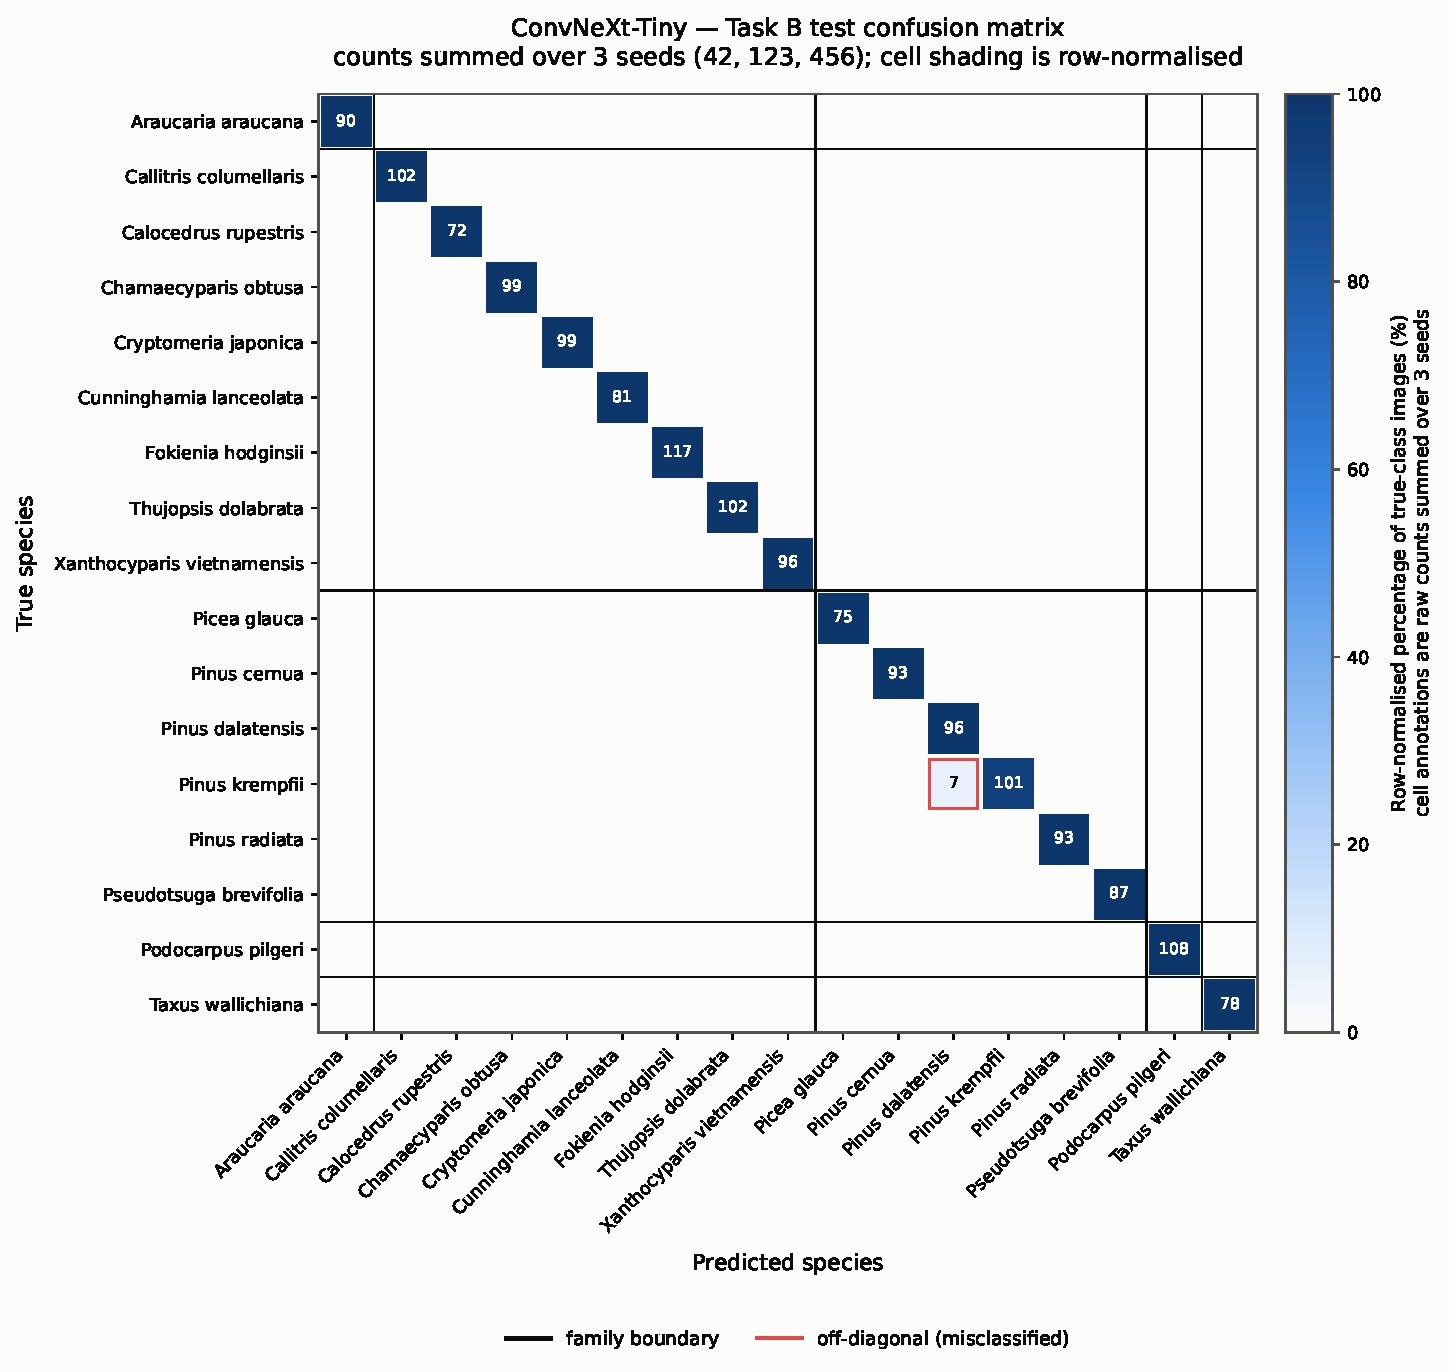
\includegraphics[width=\columnwidth]{artifact/person3/confusion/fig_confusion.pdf}
\caption{Confusion matrix for ConvNeXt-Tiny on the Task~B test set. Counts are
summed element-wise over the three main seeds (42, 123, 456), giving
$532\times3 = 1{,}596$ predictions; each seed contributes equally. Cell shading
is the row-normalised percentage of images of the true class, with the row
total of the summed counts as denominator; the annotation in each cell is the
raw summed count. Species are ordered by family and black rules mark family
boundaries. Off-diagonal cells are outlined in red. ConvNeXt-Tiny was selected
by a criterion fixed in advance --- highest mean macro-F1 over the three seeds
(Table~\ref{tab:task_b}) --- not by inspecting this matrix. The three per-seed
matrices are published alongside the aggregate so that the summation can be
checked.}
\label{fig:confusion}
\end{figure}

% Figure: per-species F1 by architecture (small multiples)
% Source   : docs/reports/experiments/phase_1b/final_b_new_recomputed/
%            20260819T043733Z/per_class_metrics.csv
% Artifacts: artifact/person3/per_class/{perclass_f1_summary.csv,
%            perclass_metadata.json, error_analysis.md}
% Run ids  : 15 (5 backbones x seeds 42/123/456), listed in perclass_metadata.json
\begin{figure}[!htbp]
\centering
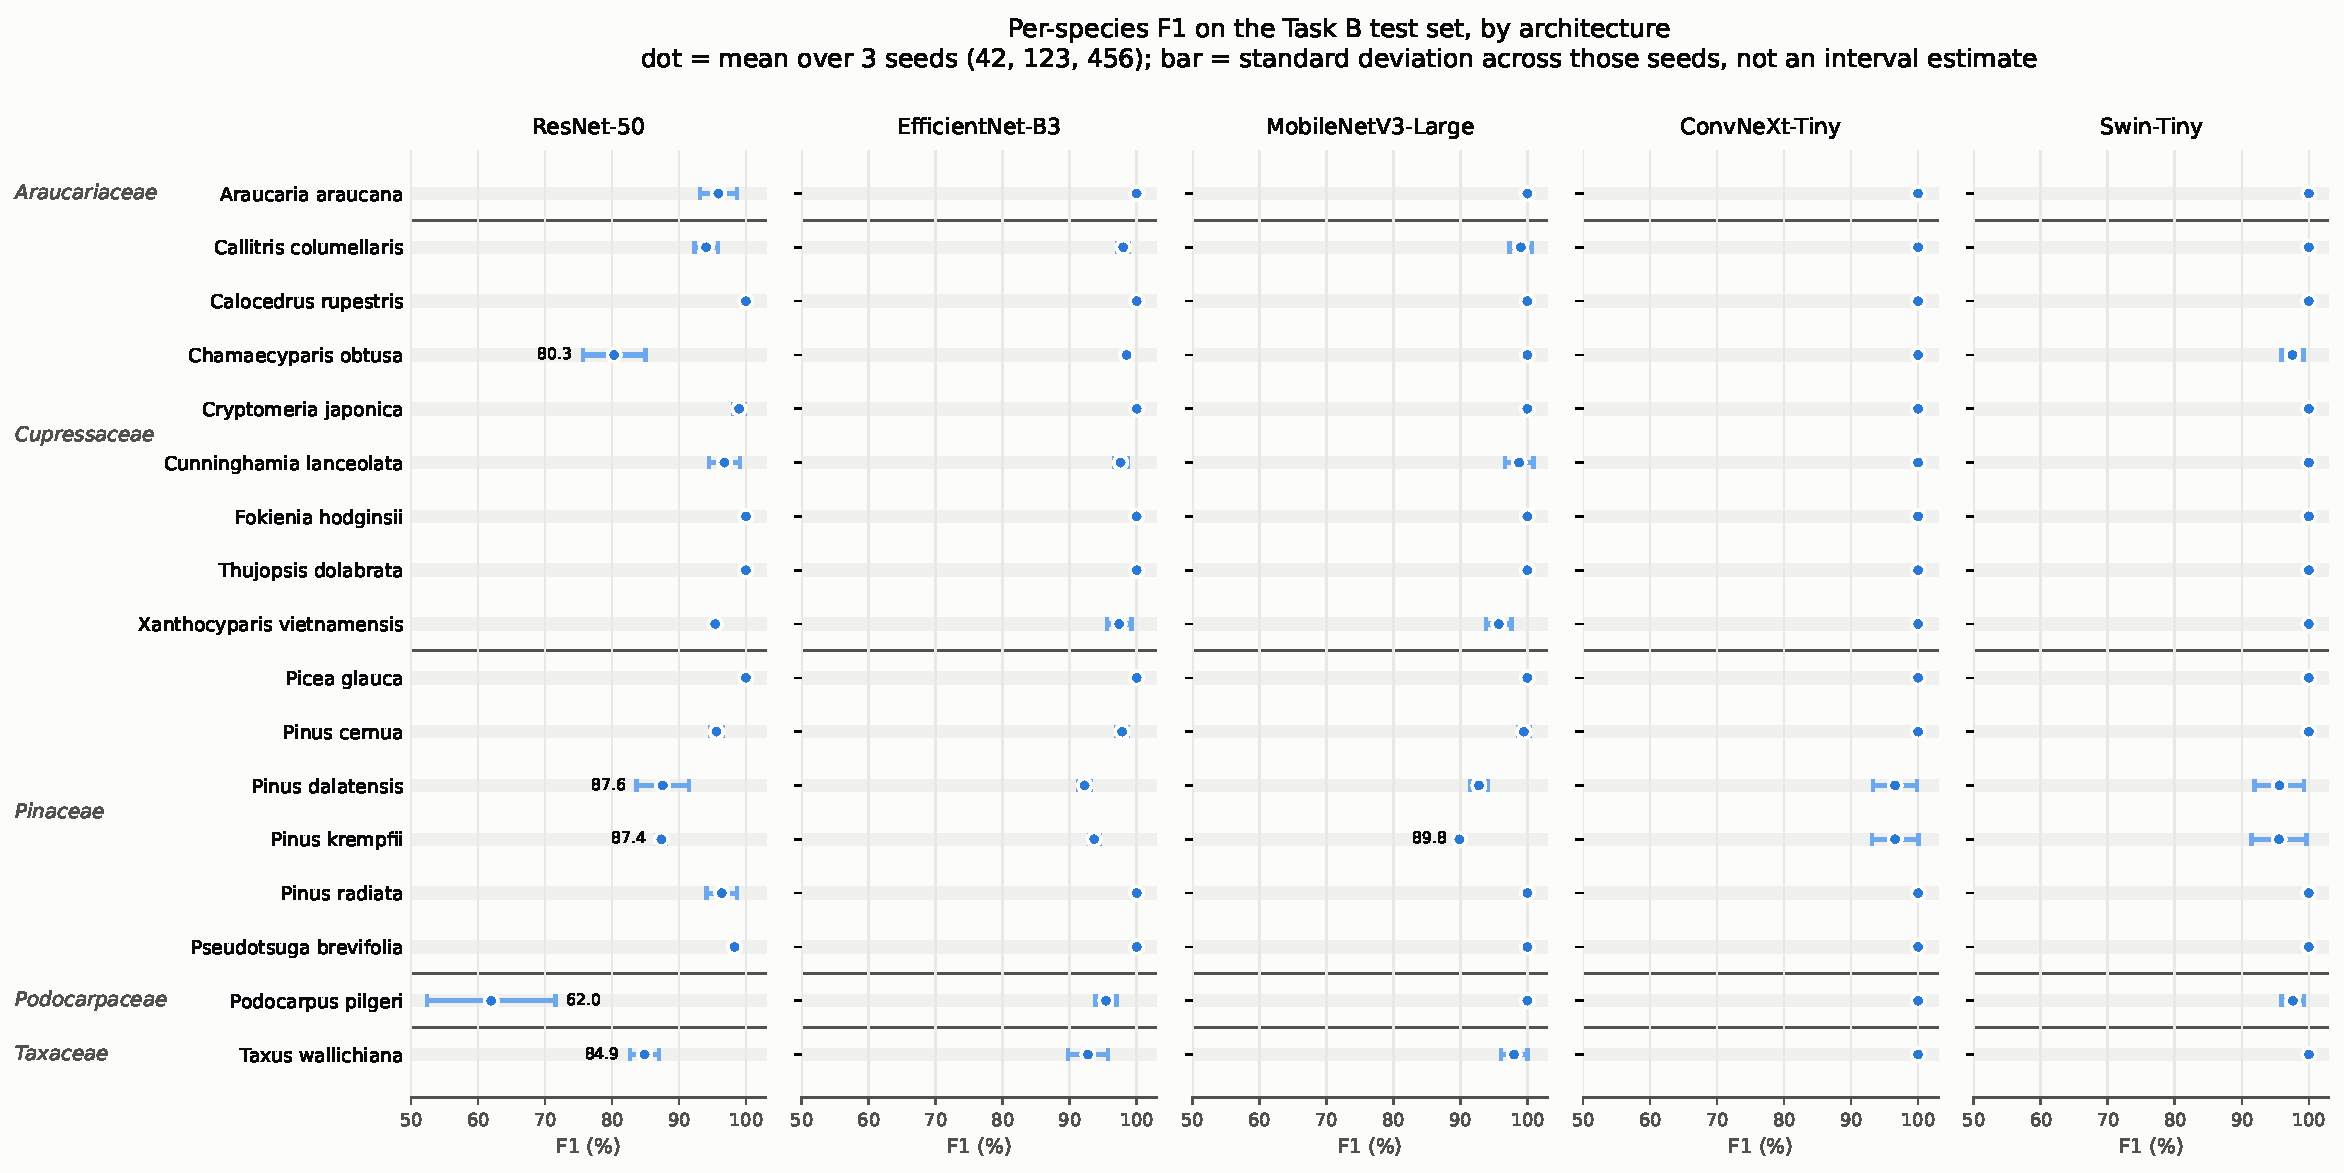
\includegraphics[width=\linewidth]{artifact/person3/per_class/fig_perclass_f1.pdf}
\caption{Per-species F1 on the Task~B test set, one panel per architecture.
Each dot is the mean over the three main seeds (42, 123, 456) and each bar is
the standard deviation across those seeds; the bar is a dispersion measure over
three runs and is not an interval estimate. Species are ordered by family, with
family blocks separated by horizontal rules and labelled at the left margin.
The horizontal axis is a position encoding and therefore does not start at
zero; values below 90\,\% are labelled directly. Architectures are separated
into panels rather than distinguished by colour, so that identity is carried by
position and panel title.}
\label{fig:perclass}
\end{figure}

% Figure: Grad-CAM, 3 architectures x 5 test images
% Source   : artifact/person1/gradcam/  (repo ManifoldsTeam/WoodID, branch p1,
%            commit d39a3f6b2cc5942e1e718c0dca86e89b0d81eb4d; see SOURCE.txt)
% Checkpoints: seed-42 runs of the same registry used elsewhere in this paper
% Manifest : artifact/person1/gradcam/{gradcam_manifest.csv,
%            sample_selection.csv, gradcam_metadata.json}
%
% NOTE ON ROW LABELS. The row labels printed in the figure follow botanical
% family and therefore show Araucariaceae for Araucaria araucana. This paper
% uses the four-family scheme of docs/references/WoodID_plan.md, in which that
% species is grouped with Pinaceae. The caption below names rows by species to
% avoid the clash; the figure itself should be regenerated with four-family
% labels before submission.
\begin{figure}[!htbp]
\centering
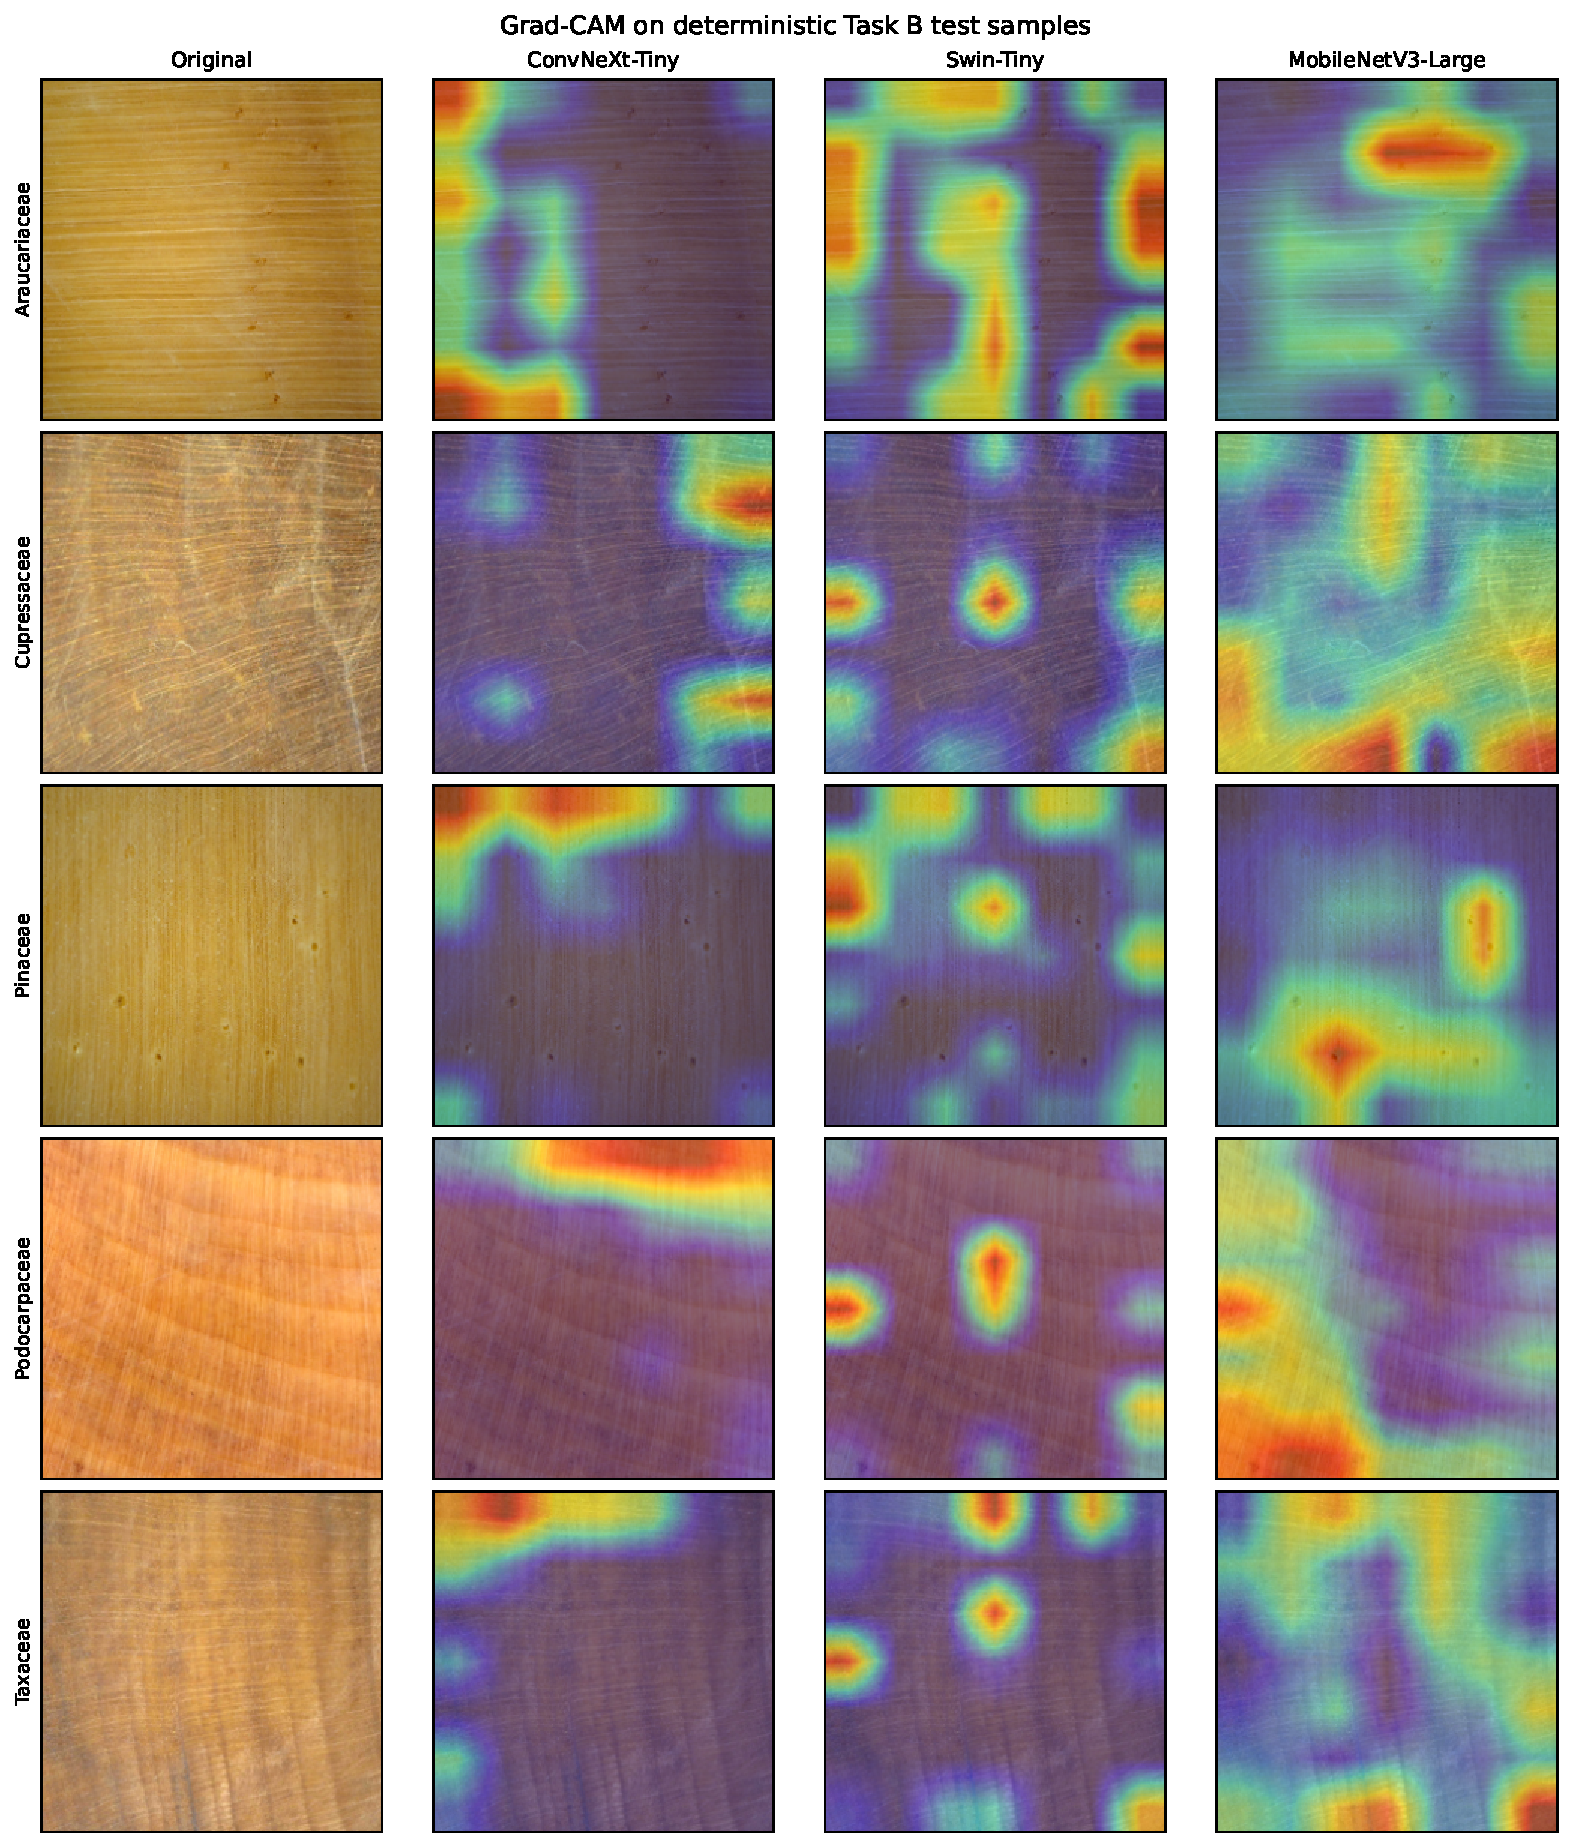
\includegraphics[width=\columnwidth]{artifact/person1/gradcam/fig_gradcam.pdf}
\caption{Grad-CAM attributions for ConvNeXt-Tiny, Swin-Tiny and
MobileNetV3-Large on five Task~B test images, one per family: \textit{Araucaria
araucana}, \textit{Calocedrus rupestris}, \textit{Pinus radiata},
\textit{Podocarpus pilgeri} and \textit{Taxus wallichiana}. Images were chosen
by a rule fixed in advance: among images classified correctly by all three
models, the one nearest the median ConvNeXt-Tiny confidence for its family,
with ties broken by image path. No image was selected for the appearance of its
heatmap. All maps come from the seed-42 checkpoints of the runs reported in
Table~\ref{tab:task_b}. Attributions are diffuse and the three architectures
highlight different regions of the same image; Grad-CAM localises gradient
support and does not by itself identify which feature is being used.}
\label{fig:gradcam}
\end{figure}

% Figure: t-SNE of ConvNeXt-Tiny pre-logit features, Task B test split
% Source   : artifact/person1/tsne/  (repo ManifoldsTeam/WoodID, branch p1,
%            commit d39a3f6b2cc5942e1e718c0dca86e89b0d81eb4d; see SOURCE.txt)
% Run id   : taskB17__main__seed_42__convnext_tiny  (same registry as Table 1)
% Artifacts: features_convnext_seed42_test.npz, tsne_embedding.csv,
%            tsne_metadata.json
\begin{figure}[!htbp]
\centering
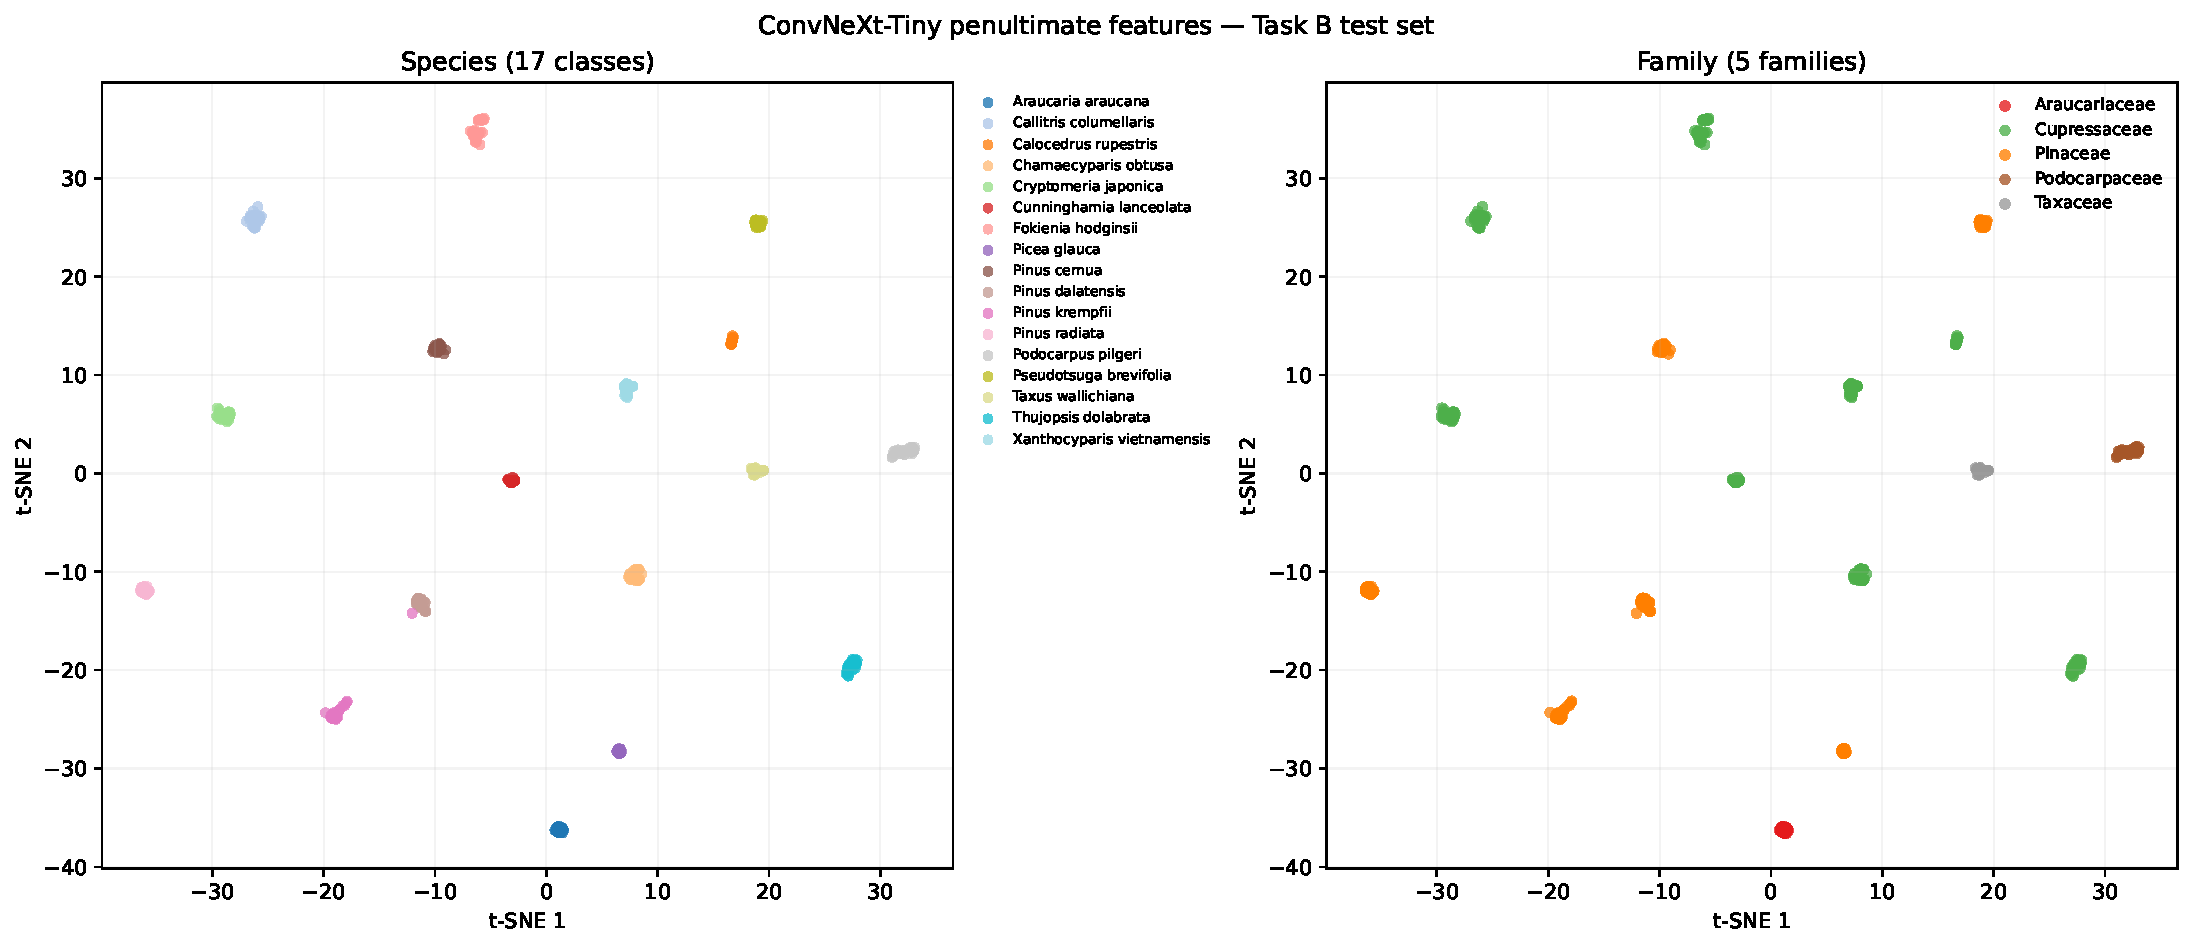
\includegraphics[width=\linewidth]{artifact/person1/tsne/fig_tsne.pdf}
\caption{Two-dimensional t-SNE embedding of ConvNeXt-Tiny features for all 532
Task~B test images, taken from the seed-42 run of
Table~\ref{tab:task_b}. Features are the 768-dimensional pre-logit activations,
standardised, reduced to 50 dimensions by PCA and then to two by t-SNE with
perplexity 30, PCA initialisation and a fixed random seed. t-SNE preserves
local neighbourhoods only: distances and cluster areas in the plot are not
metric, and the embedding is shown as a qualitative view of the representation
rather than as evidence of separability.}
\label{fig:tsne}
\end{figure}


% =====================================================================
% Section 5 — Discussion
%
% Same provenance rule as Section 4: every quantitative statement here
% resolves to a table or figure in Section 4, which resolves to registry
% 20260819T043733Z. This section adds interpretation and limitations; it
% introduces no new numbers.
%
% Dispersion is always a standard deviation over three seeds, never an
% interval estimate.
% =====================================================================

\section{Discussion}
\label{sec:discussion}

\subsection{Architecture Ranking and Seed-to-Seed Variation}
\label{sec:discussion:ranking}

The benchmark separates into two findings of very different strength, and
they should not be reported with the same confidence.

The robust finding is that ResNet-50 is not competitive on this task. Its
$92.356 \pm 1.022$\,\% accuracy sits roughly seven points below
ConvNeXt-Tiny, a gap several times its own seed-to-seed standard deviation,
and it produces 122 of the 204 errors made by all five backbones across all
seeds (Section~\ref{sec:results:perspecies}). The gap is also structural
rather than diffuse: it is concentrated in specific species where the other
four architectures are near-perfect.

The fragile finding is the ordering among the remaining four. ConvNeXt-Tiny
leads Swin-Tiny by 0.438 accuracy points while their standard deviations are
0.354 and 0.581; MobileNetV3-Large trails Swin-Tiny by 0.752 points with a
standard deviation of 0.319. These separations are of the same order as the
seed-to-seed variation, so with three seeds the ordering cannot be treated
as established, and a different seed triple could plausibly reorder them.
The defensible claim is that ConvNeXt-Tiny, Swin-Tiny and MobileNetV3-Large
all reach a comparable operating point, and that identifying a single best
architecture among them would require more seeds than this study ran.

The MobileNetV3-Large result deserves emphasis for a different reason. It
reaches within 1.19 accuracy points of the best model using 4.22\,M
parameters against 27.83\,M, and 0.22\,G MACs against 4.46\,G
(Table~\ref{tab:efficiency}) --- roughly one sixth the parameters and one
twentieth the compute. For the field-deployment scenario that motivates
macroscopic wood identification, that trade-off matters more than the
ranking at the top. The comparison is one of accuracy against static
complexity only; inference latency is not reported here, for the reason
given in Section~\ref{sec:results:efficiency}.

\subsection{What the Models Are Using: Evidence Against an Anatomical Reading}
\label{sec:discussion:shortcut}

The most consequential limitation of this benchmark is not the size of the
accuracy gaps but what the accuracies measure. The probes in
Section~\ref{sec:results:convergence} show that a Swin-Tiny trained on
$16\times16$ inputs reaches 94.361\,\% accuracy, and one trained on heavily
blurred inputs 95.677\,\%, against 99.060\,\% for the full-resolution
reference. Both destroy the anatomical structure that macroscopic wood
identification relies on, and both retain more than 95\,\% of full-image
performance.

The natural first explanation --- that the models are simply reading
colour --- is not supported: the histogram-only probe reaches 37.970\,\%.
Colour carries real signal, far above the 5.882\,\% chance level, but it
accounts for well under half of what the spatial probes achieve. The
decisive evidence is therefore spatial but low-frequency: something that
survives sixteen-fold downsampling. Broad tonal gradients, coarse
figure, overall lightness distribution and specimen-level acquisition
characteristics are all consistent with this and are not separated by the
present experiments.

Two readings remain open, and they have very different consequences. The
benign reading is that conifer species genuinely differ in bulk optical
properties at this scale, in which case the models have learned a real but
coarser cue than intended, and the benchmark measures a legitimate if
narrower task. The adverse reading is that low-frequency content carries
specimen identity --- lighting, staining, mounting, camera setup --- and
that residual specimen leakage (Section~\ref{sec:discussion:originkey})
allows it to be exploited. The two readings cannot be separated from the
present data. Distinguishing them requires evaluation on independently
acquired images, which this study does not have
(Section~\ref{sec:discussion:external}).

The consequence for reporting is direct. The headline accuracies should be
read as accuracy on this task and this corpus, not as evidence that the
models identify wood by anatomy, and the project's own probe protocol
records the benchmark as not yet released on this basis. This does not
invalidate the architecture comparison in
Section~\ref{sec:discussion:ranking}: all five backbones were trained and
evaluated under identical conditions, so their relative ordering remains a
valid comparison. It restricts what the absolute numbers may be claimed to
demonstrate.

Two further observations follow from the probes. Their retention ordering
(blur above downsampling) suggests the useful content is at a coarser scale
than $16\times16$ sampling preserves, which is a testable prediction for a
resolution sweep --- an experiment that was configured for this study but
never run (Section~\ref{sec:discussion:scope}). And the probes were trained
for 20 epochs against 50 for the main runs, so their absolute numbers are
lower bounds on what the destroyed inputs can support, which strengthens
rather than weakens the argument.

\subsection{Rotation Does Not Improve Uniformly}
\label{sec:discussion:rotation}

Discrete $90^\circ$ rotation was motivated by the observation that a
macroscopic cross-section has no canonical orientation, so rotations by
multiples of $90^\circ$ should preserve every diagnostic feature. The data
do not support the expected benefit.

The effect changes sign across architectures: positive for ResNet-50 and
EfficientNet-B3, exactly zero for MobileNetV3-Large, negative for both
ConvNeXt-Tiny and Swin-Tiny (Table~\ref{tab:ablation}). An augmentation that
genuinely encoded a property of the imaging geometry would be expected to
help, or at least not hurt, regardless of backbone. That the two strongest
models are the two that decline is the opposite of the pattern a real
invariance gain would produce.

Two readings remain open and this study cannot separate them. The
augmentation may be redundant --- the main configuration already applies
continuous $\pm30^\circ$ rotation plus horizontal and vertical flips, so
much of the orientation invariance may already be covered, leaving discrete
$90^\circ$ rotation to trade away sample diversity for nothing. Or the
deltas may simply be seed noise: four of the five magnitudes fall within
about 1.6 times the corresponding seed-to-seed standard deviation, and with
a single seed per ablation there is no way to tell a small real effect from
a favourable draw. Either way, the practical conclusion is the same:
discrete $90^\circ$ rotation should not be adopted as a default for this
task on the strength of these runs.

Label smoothing behaves differently and is worth separating. Removing it
lowers accuracy for all five backbones without exception. No individual
delta is large, and three of five are below the corresponding seed-to-seed
standard deviation, so the effect size is not established --- but the
consistency of direction across five independent architectures is the one
pattern in the ablation table that does not look like noise. Raising label
smoothing to 0.2 shows no such consistency. This is weak evidence that the
default of 0.1 is a reasonable choice, and it is not evidence that 0.1 is
optimal.

\subsection{The Single-Seed Ablation Design Is the Binding Limitation}
\label{sec:discussion:oneseed}

Every ablation in this study was trained with seed 42 only. This is the most
consequential methodological limitation of the ablation results, and it is
not repairable by analysis.

The main runs establish that seed-to-seed standard deviation on this task
ranges from 0.319 to 1.022 accuracy points depending on backbone
(Table~\ref{tab:task_b}). Of the 15 ablation deltas in
Table~\ref{tab:ablation}, 9 are smaller than the standard deviation of their
own backbone, and only one exceeds it by more than about 2.4 times. A
single-seed delta of a fraction of a point therefore carries almost no
information about the underlying effect: the measurement noise and the
effect being measured are the same size.

This has a specific consequence for how the ablation table should be read.
Individual cells should not be interpreted. What can be read is the pattern
across the row of five backbones --- a consistent sign across five
independently initialised architectures, as seen for label smoothing 0.0, is
harder to explain by seed noise than any single cell, even though each cell
alone is uninformative. This is why Section~\ref{sec:results:ablation}
reports directional consistency rather than effect magnitudes, and why no
ablation is presented as an improvement.

Repeating each ablation across the same three seeds used for the main runs
would cost 30 additional training runs and would make these comparisons
interpretable. That is the single highest-value extension to this study.

\subsection{Effect of Origin-Key Construction}
\label{sec:discussion:originkey}

The Task~B partition groups images by specimen so that all crops from one
physical wood sample fall in a single split. This matters because the source
corpus is heavily cropped: 5{,}830 images derive from 557 specimens, and
88.3\,\% of the images come from specimens contributing 24 crops or more.
Under an image-level split, a specimen with 30 crops has a probability of
about $6.9\times10^{-16}$ of avoiding the training set entirely, so
essentially every large specimen appears in training, and test images become
different crops of familiar samples rather than new samples. The earlier
image-level Task~B partition showed exactly this: 97.62\,\% of its test
images came from specimens already present in training. Accuracy measured
under that partition describes crop recognition, not species generalisation.

The specimen grouping used here removes that particular failure, but the
guarantee it provides is bounded by how the specimen key is constructed. The
key is derived from the filename: the trailing crop index is stripped and the
class name prefixed, so \texttt{3351.\ Araucaria araucana.1.(12).png} becomes
\texttt{Araucaria araucana::3351.\ Araucaria araucana.1.}. It is a naming
convention, not a specimen identifier recorded at collection time. Two
distinct consequences follow, and they are not symmetric.

Over-grouping --- two physically different specimens sharing a filename stem
and being merged into one key --- costs only split flexibility. It is
conservative and does not inflate results.

Under-grouping is the real risk. If crops of one physical specimen were
saved under different stems, for example across separate scanning sessions or
after a renaming step, the key assigns them different origins and the
grouping silently fails to separate them. Nothing in the filename can detect
this, and no independent specimen identifier exists in the corpus against
which to check it.

A dedicated audit of the key gives this concern a magnitude. Regrouping the
552 keys of the 17-class set under a coarser candidate rule yields 325
groups, a 41.1\,\% collapse: on that reading, four keys in ten are fragments
of a larger physical unit rather than units in their own right. The audit
also finds 86 sample numbers reused across species, so the numeric part of a
filename is not by itself a specimen identifier. Its stated conclusion is
that whether the key denotes a physical specimen or merely an image or view
cannot yet be determined, and that filename structure must not substitute
for verification against the collection's own records; that verification
remains outstanding. The strength of the specimen-separation claim therefore
rests on the source collection's naming discipline, which this study did not
independently verify.

Two further caveats affect what can be checked from the published artifacts.
First, roughly 19\,\% of test images carry renumbered filenames in the
deployed split, so their origin key cannot be reconstructed after the fact;
among the 81\,\% that can be reconstructed, no specimen is shared between
validation and test. Second, the registry publishes predictions for the
validation and test splits only, so the train-versus-test separation --- the
one that actually matters --- cannot be re-verified from the released
artifacts and rests on the split construction itself. Publishing the
specimen-to-split assignment alongside the registry would close this gap.

\subsection{No External or Field Validation}
\label{sec:discussion:external}

All results come from a single corpus, split internally. The models have
never been evaluated on wood imaged by a different operator, with different
equipment, under different lighting, or at a different site. Accuracy above
99\,\% should be read as accuracy on held-out specimens \emph{from this
collection}, not as an estimate of field performance.

This limit is more restrictive than it may appear, for a reason specific to
this study. The single confusion that survives in the strongest model is
between two \textit{Pinus} species, and the errors that separate ResNet-50
from the rest are concentrated in a handful of species. Both patterns are
properties of this corpus at its current size --- 24 to 39 test images per
species, drawn from a limited number of specimens per species. A different
collection could easily show a different set of difficult species without
contradicting anything reported here.

Nothing in this study supports a claim about deployment readiness. The
appropriate next step is evaluation on an independently collected set of
specimens, ideally imaged under conditions the models have not seen, before
any operational use is considered.

\subsection{Scope Decisions: Task A and the Resolution Ablation}
\label{sec:discussion:scope}

Two experiments that appear in the project plan are not reported in
Section~\ref{sec:results}, and the reasons differ.

\paragraph{Task A (family-level classification).} The family-level task used
a species-stratified split operating at the image level, the same mechanism
that produced 97.62\,\% specimen coverage in the earlier Task~B partition
(Section~\ref{sec:discussion:originkey}), applied to the same heavily cropped
corpus. Its results are therefore subject to the same leakage, and its
near-perfect family-level scores --- including one architecture at
100.000\,\% on all three seeds --- cannot be read as evidence of
generalisation to unseen specimens. Reporting Task~A alongside a
specimen-grouped Task~B would place two incomparable evaluation protocols in
one results section and invite exactly the misreading the grouped split was
built to prevent. Task~A is therefore excluded rather than reported with a
caveat. Restoring it would require rebuilding the family-level split by
specimen and retraining all 15 runs; at family level this is less likely to
run short of classes than at species level, since the three species excluded
from Task~B belong to families that retain many other specimens. Note also
that the family-level task is defined over four families, folding
\textit{Araucaria araucana} into Pinaceae, whereas the grouping used in
Section~\ref{sec:results} keeps Araucariaceae separate; the two would have to
be reconciled before the tasks could be reported side by side.

\paragraph{Input resolution.} A $384$-pixel resolution ablation was
configured but never trained; no runs for it exist in the registry. Input
resolution is consequently untested in this study. This is a genuine gap
rather than an exclusion: resolution plausibly interacts with the one
difficulty that survives in the best model, since distinguishing
\textit{P.\ krempfii} from \textit{P.\ dalatensis} may depend on fine
anatomical detail that $224$-pixel inputs do not resolve. Testing it is a
natural companion to the multi-seed ablation proposed in
Section~\ref{sec:discussion:oneseed}.

% =====================================================================
% Section 6 — Conclusion
%
% Written only after Sections 4 and 5 were complete and every table and
% figure was frozen. Introduces no number that does not already appear in
% Section 4, and no claim not already argued in Section 5.
% =====================================================================

\section{Conclusion}
\label{sec:conclusion}

This study benchmarked five deep-learning architectures on macroscopic
cross-section identification of 17 conifer species, under a partition
grouped by origin key and evaluated from a single immutable registry.

Three results are supported by the evidence presented. First, ResNet-50 is
not competitive on this task: at $92.356 \pm 1.022$\,\% accuracy it sits
roughly seven points below ConvNeXt-Tiny, a separation several times its own
seed-to-seed variation, and it accounts for 122 of the 204 errors made by
all five backbones across all seeds. Second, the remaining four architectures
are not separated by this experiment. ConvNeXt-Tiny, Swin-Tiny and
MobileNetV3-Large differ by margins comparable to the standard deviation
across three seeds, so their ordering should not be treated as established.
Third, within that group MobileNetV3-Large is the practically interesting
result: it comes within 1.19 accuracy points of the best model using one
sixth the parameters and one twentieth the compute, which is the trade-off
that matters for field deployment.

The error structure is concentrated rather than diffuse. In the strongest
model every error across three seeds is the same confusion, \textit{Pinus
krempfii} predicted as \textit{Pinus dalatensis}, and that pair is the only
one appearing in all five architectures. It is strongly asymmetric, 61
occurrences against one in the reverse direction, and it does not diminish
as capacity increases --- a pattern better read as a property of the imagery
than of any one model. By contrast the apparently large
\textit{Podocarpus pilgeri} difficulty is an artefact of pooling: 48 of its
55 occurrences come from ResNet-50 alone, and two architectures never make
that error. The same disaggregation removes the expectation that
Cupressaceae is the hardest family; over all five backbones it has the lowest
error rate of the five, though once ResNet-50 is excluded the single-species
Araucariaceae falls to zero and takes that position.

Neither augmentation ablation supports a recommendation. Discrete
$90^\circ$ rotation changes sign across architectures and helps neither of
the two strongest models. Removing label smoothing lowers accuracy in all
five backbones, which is the only directionally consistent pattern in the
ablation table, but each individual effect is small and every ablation was
trained with a single seed, so no effect size is established.

The most important qualification concerns what the accuracies measure. A
control experiment shows that a model trained on $16\times16$ inputs retains
95.3\,\% of full-image accuracy and one trained on heavily blurred inputs
96.6\,\%, while a colour-histogram-only model reaches 37.970\,\%. Anatomical
structure is destroyed at those resolutions, so the decisive evidence is
spatial but low-frequency, and the $99$\,\%-level accuracies cannot be read
as evidence that the models identify wood by anatomy. This does not
invalidate the architecture comparison, which was conducted under identical
conditions throughout, but it bounds what the absolute numbers may be
claimed to show. A specimen-key audit adds a second qualification: regrouping
the 552 origin keys under a coarser rule collapses them to 325, and whether
the key denotes a physical specimen rather than an image or view has not yet
been verified against the collection's records.

Three lines of work follow directly. Repeating each ablation across the same
three seeds as the main runs would make those comparisons interpretable at a
cost of 30 training runs. Completing the specimen-key verification against
the collection's own records would establish, rather than assume, that the
partition separates physical specimens. And evaluating on independently
acquired images --- different operator, equipment and lighting --- is the
only way to separate the benign and adverse readings of the probe results,
and the precondition for any claim about field use.

Until those are done, the defensible summary of this work is a controlled
comparison of five architectures on one corpus, with a clearly identified
species pair that resists every architecture tested, and an explicit warning
that the headline accuracy overstates what has been demonstrated about
anatomical identification.


\end{document}
